\graphicspath{{figures/chap04/}}

%\chapter{SUNIST 上光谱诊断系统和放电重复性的改善}
\chapter{SUNIST 上原子发射光谱的测量}
\label{chap:measureing-system}


本章首先介绍 SUNIST 上的诊断设备及光谱测量工作中的相关系统,然后对 SUNIST 发射光谱诊断测量系统的建立和标定以及基于重复放电的谱线测量方法进行描述,最后给出了 SUNIST 氦放电等离子体谱线测量与高斯拟合结果。其中,原子发射光谱测量系统在总装后对所使用单色仪进行了波长准确度、分辨率以及光谱响应进行了标定,通过屏蔽和隔离供电等措施对光电倍增管的谱线信号进行了噪声和基线干扰的抑制;SUNIST 实验中采用基于重复放电对氦等离子体的原子谱线进行测量,改善 SUNIST 放电的重复性不但可以获得具有重复宏观参数的等离子体放电,如气体原子激发、电离与复合等微观过程的重复性也得到了保证。

\section{SUNIST 上的诊断设备与相关系统}

\begin{figure}[H]
  \centering
  %\includegraphics[width=\textwidth]{AvailableDiagnosticsOfSUNIST-1.jpg}
  \includegraphics[width=\textwidth]{AvailableDiagnosticsOfSUNIST-14.pdf}
  \caption{SUNIST 上的诊断设备及相关系统(顶视图),修改自 \onlinecite{TanYi2013:1stA3}。}
  \label{fig:chap04:AvailableDiagnosticsOfSUNIST}
\end{figure}

SUNIST 上的诊断设备和相关系统布置情况如图 \ref{fig:chap04:AvailableDiagnosticsOfSUNIST} 所示。其中真空相关系统将在第 \ref{sec:chap04:gas-puffing-for-repeatability} 节中做详细介绍;本文在欧姆放电运行模式下进行光谱测量,而阿尔芬波与微波预电离天线为非感应等离子体启动和电流驱动研究时使用\cite{TanYi:HJBYDLZTWL:ECW,TanYi2008:Thesis,TanYi2011:NF:ECR},此处不再赘述。下面我们主要介绍 SUNIST 的诊断设备与它们在本文实验测量研究中所起的作用。

94 GHz 微波干涉仪与两台 JY 1000M-SII\cite{JY1000M} 单色仪安装在位于赤道面的小直径($d=100\,{\rm mm}$)窗口处,两台单色仪为本文原子光谱测量系统的主要设备(第 \ref{sec:chap04:spectroscopy-system} 节),微波干涉仪的诊断结果用来与本文谱线比法诊断结果进行对比(第 \ref{sec:chap04:lineratio-ne-te} 节);可移动内部静电探针和磁探针装置可以用来同时测量等离子体 $T_{\rm e}$、$N_{\rm e}$ 和磁场的径向分布,但其工作时需伸入等离子体内部,且探头尺寸较大,工作时会对等离子体造成较大影响,本文实验过程中不使用此装置;可见光探测器与高速相机安装于赤道面上的一个大尺寸($d=200\,{\rm mm}$)玻璃窗口上,可见光信号用来监测炮与炮之间放电的重复性(第 \ref{sec:chap04:repeat-shot-based-measure} 节),高速相机用来监视放电时的等离子体形态(第 \ref{sec:chap04:chord-integration} 节);极向和环向磁探针阵列用来测量等离子体的磁流体力学行为(第 \ref{sec:chap04:line-dbp10-fluctuation} 节);静电探针与单杂环信号分别可以提供边界等离子体的电子温度和密度参数与环电压信息,本文用其测量信号的标准差做为 SUNIST 等离子体放电重复性的指示(第 \ref{sec:chap04:gas-puffing-for-repeatability} 节);另外,CdZnTe 探测器测量等离子体的硬 X 射线辐射,可以为放电运行时等离子体状态判断提供参考。

\section{SUNIST 上原子发射光谱诊断系统}
\label{sec:chap04:spectroscopy-system}

\subsection{SUNIST上光谱测量系统与路径安排}

实验使用的发射光谱测量系统如图 \ref{fig:chap04:OESsystem} 所示。两条光纤通过石英玻璃窗口,在同一位置朝向相同方向收集 SUNIST 氦气放电等离子体发出的可见光,将收集到的可见光送至两台JY 1000M-SII 单色仪 Mono A 和 Mono B 的入口狭缝。经单色仪分光后,光线从单色仪的出口狭缝射出并被光电倍增管转换为光电流信号,该光电流信号经电流电压转换并被放大,最终被 SUNIST 装置上的数据采集系统进行模数转换并存入 MDSplus\cite{MDSplus:url,MDSplus:paper:1,MDSplus:paper:2} 数据库。
%电流信号,电流信号被转换为电压信号并放大,最终被数据采集器模数转换后存入 SUNIST 装置的 MDSplus\cite{MDSplus:url,MDSplus:paper:1,MDSplus:paper:2} 数据库系统。
单色仪光栅的旋转由用户通过计算机控制,数据采集系统的采样触发信号则由等离子体控制系统提供。

之所以在单色仪出口使用光电倍增管作为光探测器件,是为了保证测量的时间响应满足 SUNIST 脉冲放电等离子体(持续时间约 $10\,{\rm ms}$)的要求。虽然光电倍增管为单点探测器,但实验中两台单色仪配合使用,可以对两条谱线同时进行测量。

SUNIST 光谱测量路径如图 \ref{fig:chap04:measureing-route} 所示。在赤道面内,两条光纤通过石英玻璃窗口,在同一位置朝向真空室中心方向收集 SUNIST 氦气放电等离子体的辐射光。
%光纤接口的测量路径指向外凸的内真空室壁,这样在真空室内不安装多余部件以减少对真空本底影响的前提下,可以尽可能地减小真空室壁反射对测量的影响。
实验过程中,使用一台 94 GHz 微波干涉仪测量等离子体的平均电子密度 $\overline{N_{\rm e}}$。微波波束被聚焦后,从同一石英玻璃窗口沿图 \ref{fig:chap04:measureing-route} 中与光谱测量相同的路径打入真空室,在中心柱处被反射,被位于石英玻璃窗口前的喇叭天线接收。波束两次通过等离子体,由等离子体电子密度引起的相移需要计入两倍的沿测量路径的积分。

\begin{figure}[H]
  \centering
  \includegraphics[width=0.6\textwidth]{OESsystem.pdf}
  \caption{SUNIST 实验光谱测量设备示意图。\quad 1:氦气放电等离子体赤道面;2:石英窗口;3:光纤;4:单色仪;5:光电倍增管;6:信号放大器;7:数据采集器;8:数据库服务器;9:控制计算机;10:托卡马克与等离子体控制系统。粗实线表示光纤连接,细实线表示电信号或数据连接。图片来自 \onlinecite{xie:istw2011}。}
  \label{fig:chap04:OESsystem}
\end{figure}

\begin{figure}[H]
  \centering
  \includegraphics[width=0.5\textwidth]{instru-alignments-2.pdf}
  \caption{SUNIST 光谱测量路径图。\quad 1:SUNIST 氦气放电等离子体赤道面;2:石英玻璃窗口;3:光纤接口与准直孔;4:单色仪与 $94\,{\rm GHz}$ 微波干涉仪的测量路径;5:外真空室壁;6:外限制器边缘;7:内真空室壁与内限制器边缘。图片来自 \onlinecite{xie:wlxb}。}
  \label{fig:chap04:measureing-route}
\end{figure}


\subsection{SUNIST 上使用的单色仪参数与标定}

%\begin{table}
%\caption{JY 1000M-SII~单色仪测量汞灯谱线时不同的狭缝宽度组合}
%\label{table:chap04:different-slit-width}
%\begin{center}
%\begin{tabular}{cccccc}
%\toprule[1.5pt]
%     \multirow{2}{*}{序号} & \multicolumn{2}{c}{A~单色仪} & & \multicolumn{2}{c}{B~ 单色仪}
%     \cr\cline{2-3}\cline{5-6}
%     & 入口狭缝 ($\mu$m) & 出口狭缝 ($\mu$m) & & 入口狭缝 ($\mu$m) & 出口狭缝 ($\mu$m)\\
%\midrule[1pt]
%     1 & 10 & 10 & & 10 & 10\\
%     2 & 25 & 25 & & 25 & 10\\
%     3 & 50 & 10 & & 50 & 10\\
%     4 & 75 & 6  & & 75 & 10\\
%     5 & 100 & 6 & & 100 & 10\\
%     6 & 150 & 6 & & 150 & 10\\
%     7 & 200 & 6 & & 200 & 10\\
%\bottomrule[1.5pt]
%\end{tabular}
%\end{center}
%\end{table}

%\begin{figure}
%    \centering
%    \begin{subfigure}{0.47\columnwidth}
%        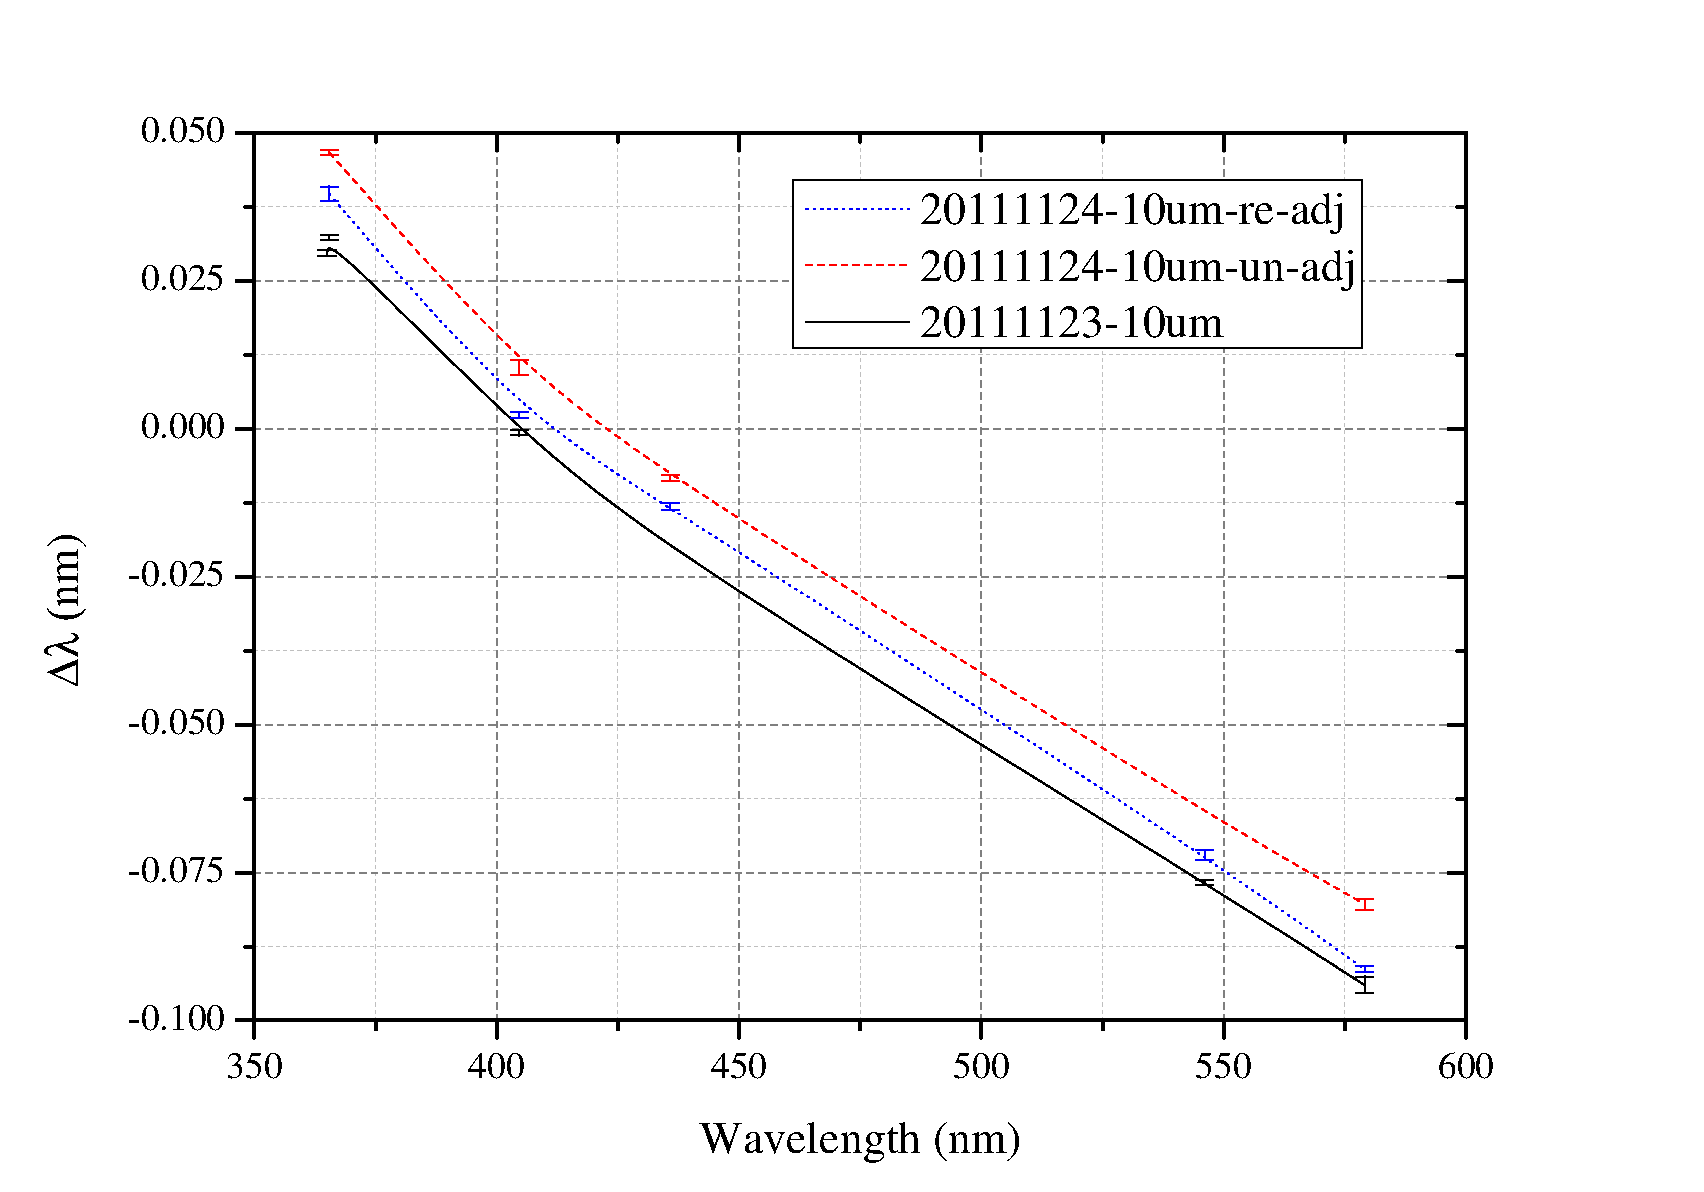
\includegraphics[width=\columnwidth]{A-delta-lambda-pre-un-re-adj-10um.pdf}
%        \caption{重新校准前后的波长准确度}%
%        \label{fig:chap03:linearity}
%    \end{subfigure}
%    %\hspace{0.05\textwidth}
%    \begin{subfigure}{0.47\columnwidth}
%        \includegraphics[width=\columnwidth]{A-FWHM-vs-slit-width.pdf}
%        \caption{不同狭缝宽度的分辨率}%
%        \label{fig:chap03:resolution}
%    \end{subfigure}
%    \caption{A 单色仪的波长准确度与谱线分辨率}%
%    \label{fig:chap03:A-linearity-and-resolution}
%\end{figure}
%
%\begin{figure}
%    \centering
%    \begin{subfigure}{0.47\columnwidth}
%        \includegraphics[width=\columnwidth]{B-delta-lambda-10um-111219.pdf}
%        \caption{重新校准前后的波长准确度}%
%        \label{fig:chap03:41S-levelabun-reldiff:1}
%    \end{subfigure}
%    %\hspace{0.05\textwidth}
%    \begin{subfigure}{0.47\columnwidth}
%        \includegraphics[width=\columnwidth]{B-FWHM-vs-slit-width.pdf}
%        \caption{不同狭缝宽度的分辨率}%
%        \label{fig:chap03:11S-levelabun-reldiff:2}
%    \end{subfigure}
%    \caption{B 单色仪的波长准确度与谱线分辨率}%
%    \label{fig:chap03:41S-levelabun-reldiff}
%\end{figure}

实验使用两台 JY 1000M-SII 单色仪进行氦放电等离子体的发射光谱测量,其基本参数如表 \ref{table:chap04:1000m_spec} 所示。实际测量中,需要根据要测量的谱线的强度调整入口和出口狭缝宽度,以达到合适的信号幅度,并在重复放电的基础上,对谱线进行扫描。实验前,使用汞灯对单色仪的波长准确度和波长分辨率进行了标定,并使用钨灯对单色仪的光谱相对响应进行标定,本节给出单色仪的各项指标标定结果。

\begin{table}[H]
\caption{JY 1000M-SII~单色仪的参数}
\label{table:chap04:1000m_spec}
\begin{center}
\begin{tabular}{ccc}
\toprule[1.5pt]
     焦距 $F_{\rm mono}$ (mm) & 色散 $D_{\rm mono}$ (nm/mm) & 分辨率 $R_{\rm mono}$ (nm) \\
%\midrule[1pt]
     $1000$ & $0.4$ & $0.004$ \\
\midrule[1pt]
      波长范围 (nm) & 光栅与中心波长 $\lambda_{\rm c, mono}$ & 入、出口狭缝 $W_{\rm ent}$、$W_{\rm ex}$ ($\mu$m) \\
%\midrule[1pt]
     $250-750$ & $2400\,{\rm g}/{\rm mm}$ @ $400\,{\rm nm}$ & $0-2000$ \\
\bottomrule[1.5pt]
\end{tabular}
\end{center}
\end{table}

\subsubsection{标定中使用的汞灯谱线}

图 \ref{fig:chap04:shape-of-Hg-lines} 所示为单色仪标定过程中使用的汞灯谱线\cite{Hg-lamp-lines}线形,其中:

\begin{figure}[H]
	\centering
    \begin{overpic}[width=0.5\textwidth]{A-shape-of-Hg-lines.pdf}
        \put(25,1){\mbox{\colorbox{white}{\hspace{1.1em} 波长差 ($\rm nm$)\quad}}}
        \put(0,42){\rotatebox{90}{\mbox{\colorbox{white}{\hspace{2em}$I$ ($\rm a.u.$)\hspace{4em}}}}}
    \end{overpic}
	%\includegraphics[width=0.6\textwidth]{A-B-FWHM-vs-wavelength-and-diff-slits-width.pdf}
    \caption{标定中汞灯的谱线线形}
	\label{fig:chap04:shape-of-Hg-lines}
\end{figure}

\begin{itemize}
	\item 汞灯窗口使用了普通光学玻璃,导致 $253.652\,{\rm nm}$ 与 $313.155\,{\rm nm}$ 的汞线强度弱。
	\item 汞的激发态能级具有精细结构,每条线均存在谱线分裂叠加的不规则形状,这对单色仪进行仪器线形(instrumental profile)或谱线分辨率的标定不利。
	\item 实际托卡马克光谱测量中使用了较宽的入口和出口狭缝,此时的仪器线形展宽远大于汞灯谱线宽度,汞灯谱线精细结构的影响可以忽略。实际操作中,将测量到的汞灯谱线宽度作为仪器展宽。
	\item $365.016\,{\rm nm}$ 与 $365.483\,{\rm nm}$ 谱线波长接近,标定过程中只取 $365.483\,{\rm nm}$ 线。
	\item $365.016\,{\rm nm}$ 与 $546.074\,{\rm nm}$ 线线形较干净,当入口和出口狭缝宽度较窄时可以用来标定仪器线形。
\end{itemize}

\subsubsection{单色仪波长准确度和分辨率标定结果}

\begin{figure}%[H]
    \centering
    \begin{subfigure}{0.8\columnwidth}
        \begin{overpic}[width=\columnwidth]{A-delta-lambda-pre-un-re-adj-10um.pdf}
            \put(35,0.5){\mbox{\colorbox{white}{\hspace{2.5em} 波长 ($\rm nm$)\hspace{2.5em}}}}
        \end{overpic}
        %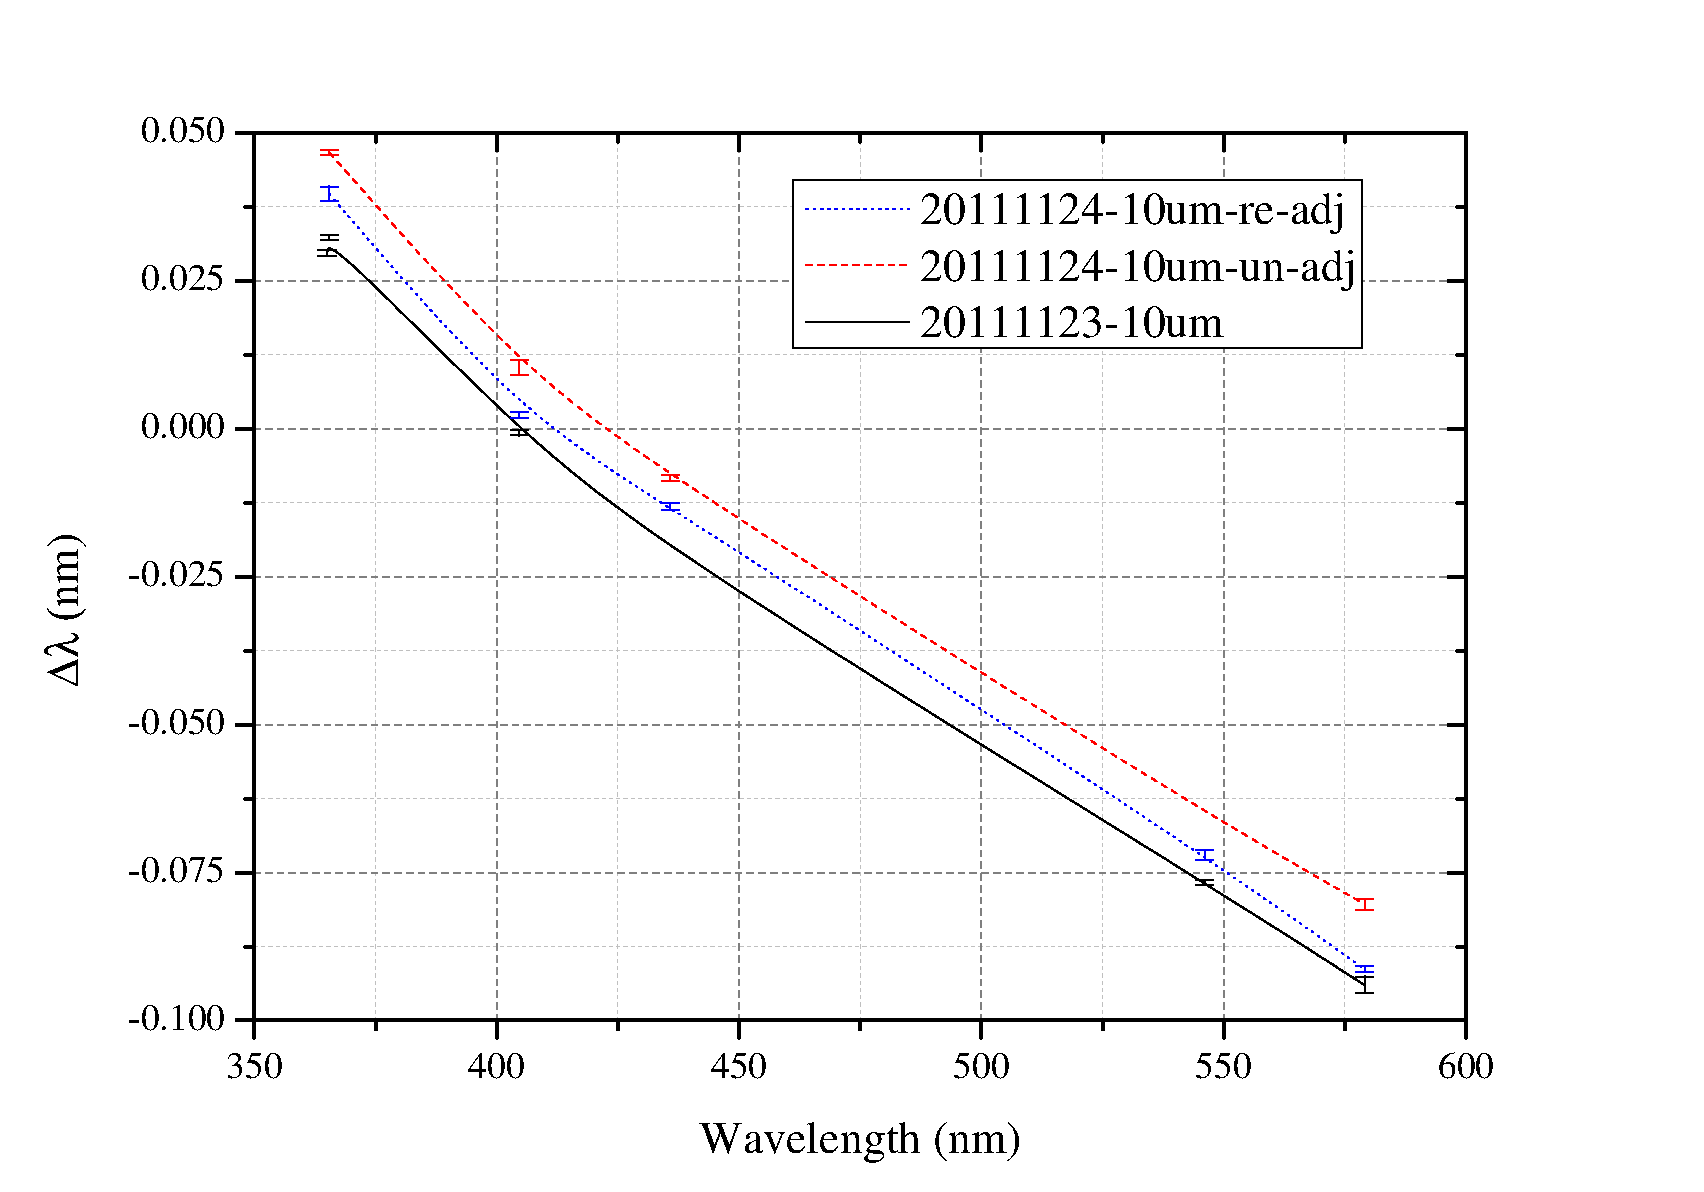
\includegraphics[width=\columnwidth]{A-delta-lambda-pre-un-re-adj-10um.pdf}
        \caption{A 单色仪波长准确度}%
        \label{fig:chap03:delta-lambda-a}
    \end{subfigure}
    \\[2em]
    %\hspace{0.03\textwidth}
    \begin{subfigure}{0.8\columnwidth}
        \begin{overpic}[width=\columnwidth]{B-delta-lambda-10um-111219.pdf}
            \put(35,0.5){\mbox{\colorbox{white}{\hspace{2.5em} 波长 ($\rm nm$)\hspace{2.5em}}}}
        \end{overpic}
        %\includegraphics[width=\columnwidth]{B-delta-lambda-10um-111219.pdf}
        \caption{B 单色仪波长准确度}%
        \label{fig:chap03:delta-lambda-b}
    \end{subfigure}
    \caption{A 单色仪与 B 单色仪校准前后的波长准确度}%
    \label{fig:chap03:delta-lambda}
\end{figure}

\begin{figure}%[H]
	\centering
    \begin{overpic}[width=0.7\textwidth]{A-B-FWHM-vs-wavelength-and-diff-slits-width.pdf}
        \put(40,0.5){\mbox{\colorbox{white}{\hspace{1.1em} 波长 ($\rm nm$)\hspace{2.5em}}}}
    \end{overpic}
	%\includegraphics[width=0.6\textwidth]{A-B-FWHM-vs-wavelength-and-diff-slits-width.pdf}
    \caption{A 单色仪与 B 单色仪在实验测量条件下测得的分辨率,两条水平虚线所示为只考虑狭缝宽度时的单色仪分辨率。括号里面的数值 $({\rm Ent}, {\rm Ex})$ 分别为入口狭缝和出口狭缝的宽度,单位为 $\mu{\rm m}$。}
	\label{fig:chap04:resolution:experiment-layout}
\end{figure}

单色仪使用光栅的闪耀波长为 $400\,{\rm nm}$,汞灯 $404.656\,{\rm nm}$ 线恰好适合用来进行单色仪的波长校准。厂家给出的波长准确度数据为 $\pm0.05\,{\rm nm}$,图 \ref{fig:chap03:delta-lambda} 所示为可见光波段两单色仪在不同波长位置的波长准确度标定结果,
%, 以及单色仪在波长标定前后和波长准确度的稳定性的测量结果.
标定过程中发现,单色仪的入口和出口狭缝宽度宽度对波长准确度的影响可以忽略。

图 \ref{fig:chap03:delta-lambda-a} 所示为 A 单色仪波长准确度在波长重新校准前后以及波长准确度在前后连续两天的稳定性测量结果。可以看出单色仪的波长准确度比厂家给出的指标略差,但处于可接受的范围内。A 单色仪的波长准确度随波长的增加线性递减,波长重新校准前后,波长误差曲线只是简单平移,说明 A 单色仪在其测量范围内的波长准确度线性较好,其波长误差范围为 $+0.05\,{\rm nm}\sim -0.10\,{\rm nm}$。随着环境温度或湿度的影响,单色仪光路会发生微弱的相对位移,这会影响单色仪的波长准确度,经过长时间的观察测量,A 单色仪波长准确度的稳定性为 $\pm0.08\,{\rm nm}$。

图 \ref{fig:chap03:delta-lambda-b} 所示为 B 单色仪波长准确度在重新校准前后以及波长准确度在相隔较长时间(约 20 天)时稳定性的测量结果。可以看出 B 单色仪的波长准确度范围为 $\pm0.10\,{\rm nm}$,比 A 单色仪稍差,且 B 波长线性也不够好,中心波长重新校准前后,波长误差校准量在不同汞线波长处不尽相同,波长越长,波长校准量越大一些。经过一段时间的观察测量,其波长准确度的稳定性为 $\pm0.12\,{\rm nm}$。

在实验中,两台单色仪的入口和出口狭缝宽度设为 $50\,\mu{\rm m}$,兼顾了测量的信噪比和光谱分辨率,图 \ref{fig:chap04:resolution:experiment-layout} 所示为实验条件下两单色仪光谱分辨率的测量结果,此时单色仪狭缝带来的仪器线形的展宽已经远大于汞灯谱线的展宽,所以在实际标定时可以将图 \ref{fig:chap04:shape-of-Hg-lines} 中汞谱线的展宽忽略。

\subsubsection{单色仪相对响应标定结果}

在实验测量中两台单色仪需要配合使用,同时测量不同的等离子体谱线辐射,并根据测量原子谱线的相对强度进行分析,所以对单色仪相对响应的整体标定不仅要进行同一单色仪对不同波长的相对响应,还要标定两个单色仪之间的相对响应。

自光辐射至最终信号采集的过程中影响光谱测量系统响应主要有:石英玻璃窗口透过率、仪器响应(包括光纤透射率、入口和出口狭缝、单色仪光路偏差、光栅反射率、光电倍增管响应等)、信号采样阻值、数据采集设备模数转换特性等。

在进行石英玻璃透射率和单色仪响应标定时使用的钨灯电流为 $800\,{\rm mA}$,此时钨灯发出温度为 $2862\,{\rm K}$ 的连续光谱黑体辐射。

图 \ref{fig:chap04:quartz-trns} 所示为石英玻璃窗口透射率标定结果,在 $360\,{\rm nm} - 750\,{\rm nm}$ 区间石英玻璃窗的透射率保持在 $90\%$ 以上且随波长均匀分布;在 $315\,{\rm nm} - 360\,{\rm nm}$ 区间透射率从 $68\% - 90\%$ 递增。氦原子谱线中只有一条 $318.775\,{\rm nm}$ 线落在透射率变化的区间内。

图 \ref{fig:chap04:response-cal-raw} 与图 \ref{fig:chap04:response-cal-result} 分布为标定 A 与 B 单色仪相对响应时测量的钨灯原始光谱与相对相应标定结果。需要注意的是:

\begin{enumerate}
  \item 标定测量时,A 与 B 的光纤入口与钨灯的相对位置要相同。
  \item A 与 B 单色仪光纤出口与狭缝的相对位置要与托卡马克实际光谱测量时保持相同。
  \item 标定测量时,为光电倍增管所加的高压要与实际光谱测量时保持相同。
  \item 每次仪器重新调试完毕后,需要对光谱响应再次进行标定。
\end{enumerate}

\begin{figure}[H]
  \centering
  \begin{subfigure}{0.55\textwidth}
  \begin{overpic}[width=\textwidth]{trns-quartz-monoA-110701.pdf}
    \put(35,0){\mbox{\colorbox{white}{\hspace{1.5em} 波长 ($\rm nm$)\hspace{2.5em}}}}
    \put(-3,30){\rotatebox{90}{\mbox{\colorbox{white}{\quad 透射率 \hspace{2em}}}}}
  \end{overpic}
  \caption{石英玻璃窗口透射率}
  \label{fig:chap04:quartz-trns}
  \end{subfigure}
  \\
  \begin{subfigure}{0.48\textwidth}
  \begin{overpic}[width=\textwidth]{rspn-rawdata-A-B-120523.pdf}
    \put(35,-1){\mbox{\colorbox{white}{\hspace{1.2em} 波长 ($\rm nm$)\hspace{2.5em}}}}
    \put(-2,30){\rotatebox{90}{\mbox{\colorbox{white}{\quad $I$ ($\mu{\rm A}$)\quad}}}}
  \end{overpic}
  \caption{测量的钨灯连续谱数据}
  \label{fig:chap04:response-cal-raw}
  \end{subfigure}
  \hspace{0.02\textwidth}
  \begin{subfigure}{0.48\textwidth}
  \begin{overpic}[width=\textwidth]{rspnMonoAB-120523-wo-quartz-Radiance.pdf}
    \put(35,-1){\mbox{\colorbox{white}{\hspace{1.2em} 波长 ($\rm nm$)\hspace{2.5em}}}}
    \put(-3,15){\rotatebox{90}{\mbox{\colorbox{white}{$R_{\rm A}$、$R_{\rm B}$ 或 $R_{\rm A}/R_{\rm B}$ (${\rm a.u.}$)}}}}
  \end{overpic}
  \caption{相对响应标定结果}
  \label{fig:chap04:response-cal-result}
  \end{subfigure}
  %\includegraphics[width=0.6\textwidth]{rspnMonoAB-120523-wo-quartz-Radiance.pdf}
  \caption{A 单色仪与 B 单色仪相对响应标定结果}
  \label{fig:chap04:response-cal}
\end{figure}

造成 A 与 B 单色仪相对响应不同的因素很多,比如光纤透过率、光栅反射率、单色仪光路偏差等,但主要的原因应该为两单色仪使用的光电倍增管响应差异以及单色仪入口处狭缝与光纤的耦合情况。所用钨灯在 $315\,{\rm nm} - 350\,{\rm nm}$ 范围内的辐射很弱,此波长范围内无法获得有足够信噪比的原始数据,单色仪的相对响应标定数据也不可靠,这样氦的 $318.775\,{\rm nm}$ 线无法获得可信的单色仪相对响应数据,在进行相对强度分析时此谱线将不能使用。

\subsection{光电倍增管信号降噪与基线干扰的消除}

\begin{figure}[H]
	\centering
    \begin{subfigure}{0.48\columnwidth}
        \begin{overpic}[width=\columnwidth]{sampleRNoiseEffect.pdf}
            \put(32,0){\mbox{\colorbox{white}{\small\hspace{1em} 时间 ($\rm ms$)}}}
        \end{overpic}
        %\includegraphics[width=\columnwidth]{sampleRNoiseEffect.pdf}
        \caption{信号噪声与采样电阻的关系}%
        \label{fig:chap04:signal-noise:sample-R-noise-effect}
    \end{subfigure}
    \hspace{0.02\textwidth}
    \begin{subfigure}{0.48\columnwidth}
        \begin{overpic}[width=\columnwidth]{cableSuroundLayerGroundEffect.pdf}
            \put(32,0){\mbox{\colorbox{white}{\small\hspace{1em} 时间 ($\rm ms$)}}}
        \end{overpic}
        %\includegraphics[width=\columnwidth]{cableSuroundLayerGroundEffect.pdf}
        \caption{外皮接地屏蔽双绞信号线的降噪效果}%
        \label{fig:chap04:signal-noise:cable-suroundlayer-ground-effect}
    \end{subfigure}
	\caption{单色仪输出信号的噪声与噪声消除}
	\label{fig:chap04:signal-noise}
\end{figure}

\begin{figure}
  \centering
  \begin{overpic}[width=0.7\textwidth]{AH72_BH32.pdf}
    \put(38,1){\mbox{\colorbox{white}{\hspace{1em} 时间 ($\rm ms$)}}}
  \end{overpic}
  %\includegraphics[width=0.7\textwidth]{AH72_BH32.pdf}
  \caption{测量设备整体隔离供电消除基线干扰。A:扫描 H(7-2) 线;B:扫描 H$_\alpha$ 线。}
  \label{fig:chap04:ripple-isolate}
\end{figure}

等离子体辐射的可见光经单色仪分光从出口狭缝射出,经光电倍增管转换检测为微弱电流信号,电流信号幅度与光强成正比。因为光电倍增管的时间响应快速,为了不损失信号的频率响应,在光电倍增管阳极处直接串联采样电阻将电流信号转化为电压信号,以减小电路杂散参数对信号带宽的影响。

实际测量中发现采样电阻阻值越大,暗信号\pozhehao 即单色仪不进光时信号\pozhehao 的噪声越强,如图\ref{fig:chap04:signal-noise:sample-R-noise-effect} 所示。采用具有屏蔽网的双绞线传输信号至采集器会明显降低信号的噪声水平,如图 \ref{fig:chap04:signal-noise:cable-suroundlayer-ground-effect} 所示。同时,A 与 B 单色仪信号基线仍存在干扰,尤其 B 单色仪的基线受到放电时 SUNIST 托卡马克磁场线圈与供电电容器放电过程的影响,基线出现了非常剧烈的抖动。通过一一排除硬 X 射线、杂散电磁场、信号传输线以及数据采集器自身干扰后,发现此干扰这可能是由于放电末期,等离子体与真空室壁强烈相互作用,导致装置电势波动,单色仪供电电源受到影响,从而引起信号的波动干扰引起的。通过将包括控制计算机、单色仪等相关测量设备供电与市电隔离,并为光电倍增管制作独立的锂离子电池电源,此基线干扰可以很好的消除,同时 A 单色仪的信号基线也有明显改善,如图 \ref{fig:chap04:ripple-isolate} 所示。

\section{SUNIST 原子发射光谱测量手段的建立}%和前提条件的满足}

\subsection{SUNIST 上基于重复放电的谱线测量}
\label{sec:chap04:repeat-shot-based-measure}
%\subsection{SUNIST 氦放电等离子体的原子光谱测量}

\begin{figure}%[H]
  \centering
  \begin{overpic}[width=0.8\textwidth]{he-lines-shape-intensity-10-8-6-for-thesis.pdf}
    \put(42,32.3){\colorbox{white}{\color{white}$\blacksquare$}}
    \put(39,32.1){\mbox{{时间}}}%\colorbox{white}
  \end{overpic}
  %\includegraphics[width=0.7\textwidth]{AH72_BH32.pdf}
  \caption{基于重复放电的 SUNIST 氦等离子体原子发射光谱测量。上图:光谱测量时所有放电的等离子体电流 $I_{\rm p}$ 和可见光信号 ${\rm V.L.}$;中图:以 $504.8\,{\rm nm}$、$492.2\,{\rm nm}$ 和 $447.1\,{\rm nm}$ 线为例,谱线相对强度 $I$ 随时间的变化;下图:$37.49\,{\rm ms}$ 时刻,三条谱线的线形测量结果。}
  \label{fig:chap04:he-lines-shape-intensity}
\end{figure}

虽然 SUNIST 已经开展了一些非感应式的电流启动和维持研究\cite{TanYi:HJBYDLZTWL:ECW,TanYi2008:Thesis},现阶段欧姆放电仍然是进行物理研究时的主要运行模式。由于 SUNIST 的中心柱空间受到了极大限制,欧姆场提供的伏秒数仅能维持约 $10\,{\rm ms}$ 的等离子体,能用于进行各项研究的等离子体电流平顶段则更短,所以,在 SUNIST 中一般进行基于重复放电的多次测量,以获得感兴趣测量物理量随某个维度的变化数据\cite{WangWH2005:PPCF:Edge,HeYexi2006:PST:startup,XieHQ:2011:ISTW}。

本文实验测量中使用了两台单色仪,每次放电只能同时测量两条谱线线形上的一个数据点,实验中采用了多炮放电重复测量的方法,对表 \ref{table:chap03:helines-mod} 中的谱线形状进行了时间分辨测量。图 \ref{fig:chap04:he-lines-shape-intensity} 显示了在放电平顶段,多炮重复放电测量中等离子体电流、可见光、氦原子谱线辐射强度以及在 $37.49\,{\rm ms}$ 时刻三条谱线比法使用谱线的波形测量结果。谱线的相对强度是通过对氦原子的谱线线形进行高斯拟合拟合并积分得到的(详见第 \ref{sec:chap04:line-measure-result} 节)。
%这些谱线来自于主量子数 的两个单态能级和一个三态能级,其中单态谱线的强度比 对 敏感,单态谱线与三态谱线的强度比 对 敏感,两谱线比结合可以同时确定 和 。 同时我们注意到 线的强度较弱,该谱线强度的涨落造成了谱线比的涨落,从而导致图4(a)所示的等离子体参数的涨落。

本文 SUNIST 上谱线比法诊断等离子体 $T_{\rm e}$ 和 $N_{\rm e}$ 的测量研究中,主要对放电过程中等离子体的 $T_{\rm e}$ 和 $N_{\rm e}$ 参数以及原子反应过程的重复性提出了要求。在重复放电测量中,每炮放电等离子体 $N_{\rm e}$ 之间的误差要求小于谱线比法的测量误差,由图 \ref{fig:chap04:lineratio-te-ne}(b) 可得 $s_{N_{\rm e}}\ll 1.0\times10^{12}\,{\rm cm}^{-3}$;对于等离子体内部原子反应过程的重复性,受限于 SUNIST 现有的诊断手段,我们只能通过等离子体电流 $I_{\rm p}$、可见光信号 ${\rm V.L.}$、放电时气压 $p_{\rm gas}$ 以及单杂环(环电压)信号 $V_{\rm FL}$ 来保证。

\graphicspath{{figures/appendix-gaspuffing/}}
\subsection{SUNIST 放电重复性的改善}
\label{sec:chap04:gas-puffing-for-repeatability}
%\subsection{进气时序影响 SUNIST 放电重复性}

能够影响 SUNIST 放电重复性的控制手段主要包括环向、垂直、欧姆磁场的电流及投入时间和进气脉冲的宽度与时序等。在实际运行过程中,三个磁场的电流和投入时间这些电学参数可以精确控制,其重复性可以保证。经充分地放电锻炼后,真空室壁条件处于稳定,放电时的杂质行为及粒子循环等过程\cite{Belyakov2003:InpurityToPlasma:TRANSMAK} 趋于稳定。但是控制压电阀门进气的电源受到了工频干扰,其电压输出存在明显的纹波,这会影响压电阀门控制的进气流速。另外,放电过程中,SUNIST 真空室内的气压处于动态变化过程中,不易得到控制。实际运行中,我们观察到进气脉冲对 SUNIST 放电重复性具有明显影响\cite{TanYi2011:NF:ECR,HeYexi2006:PST:startup}。 在其他装置上同样也观察到了进气对放电的影响,如在 MAST\cite{Carolan:2002:MASTgaspufftoLHmode} 与 NSTX\cite{Maingi2004:PPCF:NSTXgaspufftoLHmode} 上进气位置可以影响低 -- 高模约束模式的转换过程,在不同的气压下,气体击穿时对环向感应电场的要求也是不同的\cite{Chattopa1996:SINP:breakdown,Antonio2001:TCABR:breakdown}。 所以,有必要改进 SUNIST 的进气脉冲控制,进行气压分布研究,改善放电的重复性\cite{xie:pst}。这样不但可以获得具有重复宏观参数\pozhehao 如等离子体电流等\pozhehao 的等离子体放电,而且如气体原子激发、电离与复合等微观过程的重复性也能得到保证,有助于后续光谱实验研究中实现基于重复放电的逐炮测量。

\subsubsection{用于进气时序研究的真空相关硬件系统}
\label{subsec:vv-related-parts}

为了实现稳定的进气流速和研究进气脉冲后真空室内的压强变化,本文为 SUNIST 设计安装了相应的信号采集电路并重新制作了压电陶瓷阀门控制电源。真空相关硬件系统包括真空室及相关部件、气压信号采集电路和压电阀控制电源三部分,图 \ref{fig:chap04:vacuum-system} 为 SUNIST 用于进气时序研究的真空相关硬件系统示意图。

\begin{figure}
  \centering
  \includegraphics[width=0.8\textwidth]{vacuum-system-4.pdf}
  \caption{SUNIST 真空相关硬件系统示意图}
  \label{fig:chap04:vacuum-system}
\end{figure}

1)真空室及相关部件

图 \ref{fig:chap04:topview-vacuum-vessel} 为 SUNIST 真空室顶视图。SUNIST 使用一台分子泵做为主抽气泵,主抽气窗口上安装有直径 $d=200\,{\rm mm}$,长 $L=900\,{\rm mm}$ 的主抽气管道,在主抽气管道中间安装有一只 ZJ-27\cite{ZJ-27} 热阴极离子真空规管。在 SUNIST 真空室上部进气窗口处,通过一条直径为 $d=50\,{\rm mm}$,长为 $L=300\,{\rm mm}$ 的充气管道安装有一只 PEV-1\cite{PEV-1} 压电陶瓷阀门。其中,主抽气窗口与充气窗口沿环向呈 $120^\circ$ 角。当主抽气分子泵停止运行时,使用一台溅射离子泵维持真空本底。

\begin{figure}
  \centering
  \includegraphics[width=0.6\textwidth]{topview-vacuum-vessel.pdf}
  \caption{SUNIST 真空室顶视图,修改自 \onlinecite{TanYi2013:1stA3}。}
  \label{fig:chap04:topview-vacuum-vessel}
\end{figure}


2)气压信号采集电路

电离规控制器有三个作用:a)为电离规管提供电源;b)将电离规管输出处理为气压信号,并通过数码显示管以 $1\,{\rm Hz}$ 的频率慢速显示;c)输出快速气压模拟量信号。真空室气压快速信号可以用来分析真空室内的气压流动,以获得对脉冲进气后真空室内部气压分布变化情况,选择合适的进气脉冲宽度和时序以改善放电重复性。

\begin{figure}%[H]
  \centering
  \rotatebox{270}{\includegraphics[height=0.8\textwidth]{50Hz-notch-filter.pdf}}
  \caption{SUNIST 上使用的去除气压信号中工频干扰的无源双 T 陷波器电路图}
  \label{fig:chap04:50HzNotchFilter}
\end{figure}

然而,真空规控制器输出的气压信号受到强烈的 $50\,{\rm Hz}$ 电网工频干扰。要去除电源线带来的干扰,可以串入无源双 T 陷波器(passive twin-T notch filter,图 \ref{fig:chap04:50HzNotchFilter}),其传输特性计算结果如图 \ref{fig:chap04:BodeDiagram50HzNotchFilter} 所示,由于使用的电阻和电容实际值与设计有偏差,陷波器的中心截止频率为 $50.9\,{\rm Hz}$,实际测量结果显示,该陷波器可以很好的消除气压信号中的工频干扰(图 \ref{fig:chap04:50hz-trapping})。气压信号的变化频率为 $10\,{\rm Hz}$ 量级,陷波器会在此频率的信号上引起约 $70^\circ$ 的相位延迟(图 \ref{fig:chap04:BodeDiagram50HzNotchFilter}(b)),图 \ref{fig:chap04:50hz-trapping} 显示的加入陷波器后引起的 $\sim21\,{\rm ms}$ 信号延迟与陷波器的传输特性计算结果相吻合。

\begin{figure}
  \centering
  \begin{overpic}[width=0.7\textwidth]{50Hz-notch-filter-Bode-Diagram.pdf}
    \put(42,0.7){\mbox{\colorbox{white}{\quad 频率 (Hz) \quad}}}
    \put(0.7, 18.5){\rotatebox{90}{\mbox{\colorbox{white}{相位 ($^\circ$)}}}}
    \put(0.7, 49){\rotatebox{90}{\mbox{\colorbox{white}{\quad 增益\quad}}}}
  \end{overpic}
  \caption{双 T 陷波器伯德图(bode diagram)}
  \label{fig:chap04:BodeDiagram50HzNotchFilter}
\end{figure}

\begin{figure}
  \centering
  \begin{overpic}[width=0.7\textwidth]{50hz_trapping.pdf}
    \put(42,0){\mbox{\colorbox{white}{\small 时间 (${\rm ms}$)}}}
    %\put(63, 38){\mbox{\colorbox{white}{\small 平滑处理}}}
  \end{overpic}
  \caption{气压信号 $p_{\rm gas}$ 在加陷波器(w/ twin-T)与不加陷波器(w/o twin-T)情况下的测量结果,进气脉冲以灰度条表示。}
  \label{fig:chap04:50hz-trapping}
\end{figure}

放电过程中,气压信号的地电位会随着真空室浮动,我们在真空测量系统与数据采集系统之间加入隔离运放,不但可以将气压信号地电位与数据采集系统隔离,保护数据采集系统,而且可以用其驱动气压测量设备与数据采集系统之间的长导线。

电离规控制器输出的信号幅值与气压关系标定结果在图 \ref{fig:chap04:GasSignalCalibration} 中画出,拟合结果为:
\begin{equation}
  p_{\rm gas}(10^{-3}\,{\rm Pa})=20.5670\times S_{\rm gas}({\rm V})-0.9683
  \label{eq:chap04:gas-signal-calibration}
\end{equation}
其中,$S_{\rm gas}$ 为气压信号测量幅值。

\begin{figure}
  \centering
  \begin{overpic}[width=0.7\textwidth]{gas-pressure-to-signal-calibration.pdf}
    \put(42,0.7){\mbox{\colorbox{white}{气压信号 (V)}}}
    \put(0, 20){\rotatebox{90}{\mbox{\colorbox{white}{真空室气压值}}}}
    \put(66, 12){\mbox{\colorbox{white}{\small 数据拟合\hspace{1cm}}}}
    \put(66, 16.5){\mbox{\colorbox{white}{\small 实验数据\hspace{1.5cm}}}}
  \end{overpic}
  \caption{SUNIST 气压信号幅度标定结果}
  \label{fig:chap04:GasSignalCalibration}
\end{figure}

3)压电阀控制电源系统

共有两个压电阀控制电源投入使用:主控制器与新设计安装的脉冲控制器。主控制器可以工作在本地和远程模式。在本地工作模式下,主控制器可以手动和自动控制压电阀的进气,其中手动控制只在调节测试情况下使用,自动进气由电离规控制器的继电器反馈迂回开合完成,可以自动控制真空室内的气压在一个预设范围内浮动,这种工作模式仅在辉光放电清洗真空室时使用。对于远程模式,进气脉冲由托卡马克与等离子体控制系统(tokamak and plasama control system, PCS)触发控制,进气脉冲的时序与长度调节精度可达 $0.01\,{\rm ms}$。然而,就像前面提到的,主控制器由市电直接供电,其输出中含有较大的纹波,这个纹波电压在辉光放电时的慢速粗略充气中并不会产生明显影响,但是对于托卡马克放电实验时的精确进气却不是不可接受的。所以,我们新设计并安装了一个脉冲进气控制器,该控制器由串联的干电池供电,该脉冲控制器的控制电压输出纹波可以忽略。压电阀的进气速率由所加控制电压调节,使用无纹波的脉冲控制器可以在炮与炮之间以相同的稳定进气速率对 SUNIST 真空室充气,最终,每次放电时可以保证冲入的气体量精确相同。脉冲控制器的输出同样是由 PCS 控制的。

\subsubsection{真空室内气体流动模拟}

尽管已经实现了放电时气压的变化快速信号测量,但是真空室内的气压分布瞬态过程确是难以测量的,通过真空室内气体的流动模拟,可以实现气压分布的瞬态过程分析。

SUNIST 放电时的充气气压范围为 $2\times10^{-3}\,{\rm Pa}$ 至 $1\times10^{-2}\,{\rm Pa}$。此气压下气体分子的平均自由程(室温下,对于氢气为 $7.9\,{\rm m}-1.6\,{\rm m}$)大于真空室尺度,常规连续流体模拟手段对于 SUNIST 真空室内的稀薄气体不再适用。Molflow+\cite{Molflow:paper,Molflow-url} 软件利用探测粒子蒙特卡洛模拟方法(test-particle Monte Carlo method,TPMC),可以实现稀薄气体流动模拟,实现如气压分布、有效抽气速度、器壁吸附速率等参数的计算。

图 \ref{fig:chap04:vv-3d-model} 所示为用于气体流动模拟的 SUNIST 真空室三维模型。在模型中,除了进气和主抽气窗口外的其他窗口以及真空室内的限制器都被移除,实际装置上的充气与抽气管道内的气体流动与气压分布对我们的研究并不重要,所以这些管道也一并移除。

\begin{figure}%[H]
  \centering
  \includegraphics[width=0.6\textwidth]{moflow-vessel.pdf}
  \caption{Molflow+ 模拟使用的 SUNIST 真空室三维模型。共计算了五个截面的气压分布:A)主抽气口截面;B)充气口截面;C)位于赤道面以上,与赤道面平行的环向真空室截面;D)通过充气口中心的极向真空室截面;E)通过主抽气口中心的极向真空室截面。}
  \label{fig:chap04:vv-3d-model}
\end{figure}

A 平面的脉冲出气速率和时长设为 $50\,{\rm Pa}\cdot{\rm L}/{\rm s}$ 和 $100\,{\rm ms}$,B 平面的抽气速率设为 $1200\,{\rm Pa}\cdot{\rm L}/{\rm s}$。模拟中通过对穿过感兴趣截面或在感兴趣截面处反射的粒子数进行统计,完成该截面上的气压分布计算。在放电持续时间很长的托卡马克中,来自壁循环的气体对维持真空室内的粒子数起到重要作用,但是在对 SUNIST 的模拟中,基于以下几点考虑:a)SUNIST的放电时间很短,b)真空室壁材料使用不锈钢并做了很好的抛光处理,c)实验前都会对真空室进行烘烤和辉光放电清洗,d)分子泵的抽速远大于真空室壁的充气速率,e)在长时间连续放电时,壁吸附和解析过程达到平衡,真空室壁设为无壁吸附和解析的漫反射面。

\begin{figure}%[H]
    \centering
    \begin{subfigure}{0.465\columnwidth}
        \begin{overpic}[width=\columnwidth]{fig_6_a.pdf}
          \put(33,1.5){\mbox{\colorbox{white}{\quad 时间}}}
        \end{overpic}
        \caption{}%
        \label{fig:simulation:4}
    \end{subfigure}
    \begin{subfigure}{0.45\columnwidth}
        \fbox{\includegraphics[width=\columnwidth]{fig_6_b.pdf}}
        \caption{}%
        \label{fig:simulation:1}
    \end{subfigure}
    \begin{subfigure}{0.45\columnwidth}
        \fbox{\includegraphics[width=\columnwidth]{fig_6_c.pdf}}
        \caption{}%
        \label{fig:simulation:2}
    \end{subfigure}
    \hspace{1em}
    \begin{subfigure}{0.45\columnwidth}
        \fbox{\includegraphics[width=\columnwidth]{fig_6_d.pdf}}
        \caption{}%
        \label{fig:simulation:3}
    \end{subfigure}
    \caption{主抽气口处(图 \ref{fig:chap04:vv-3d-model} 中 C 截面)平均气压和近赤道截面(图 \ref{fig:chap04:vv-3d-model} 中 E 截面)气压分布的 Molflow+ 模拟结果。
    图\ref{fig:simulation:1}、\ref{fig:simulation:2} 和 \ref{fig:simulation:3} 分别对应
    图 \ref{fig:simulation:4} 中的(1)、(2) 和 (3) 时刻。具有与模拟相同进气量的气压实际测量曲线也在图 \ref{fig:simulation:4} 中画出。图片来自 \onlinecite{xie:pst}。}%
    \label{fig:simulation}
\end{figure}

主抽气口处(图 \ref{fig:chap04:vv-3d-model} 中 B 截面)平均气压和近赤道截面(图 \ref{fig:chap04:vv-3d-model} 中 C 截面)气压分布的模拟结果在图 \ref{fig:simulation} 中画出。在气压上升阶段,模拟计算的出气口处气压值与实际测量曲线相符(图 \ref{fig:simulation:4})。当进气结束时,模拟气压值呈指数下降趋势,但是气压测量值中存在一个准稳态的平顶区。这是因为在实际装置上,压电阀与进气窗口之间 $300\,{\rm mm}$ 长的充气管道起到了缓冲作用,在进气停止后,管道内的较高压强气体仍然向真空室内充气。

进气脉冲过程中,气压处于快速上升阶段,此时气压在大环方向具有明显的分布不均(图
\ref{fig:simulation:1}),但是,由于气体分子的自由程大于真空室尺度,气体分子会在瞬间到达真空室的各个地方。中心柱也会在一定程度上对气压分布产生影响。当进气脉冲结束时,气压值达到最高,大环方向大尺度的气压不均匀性消失(图 \ref{fig:simulation:2}),但仍然存在小尺度上的气压分布不均匀性。一段时间后,真空室内的气压分布变得均匀(图 \ref{fig:simulation:3})。

真空室内气压流动模拟结果显示,气压分布的演化与气压信号可以紧密联系起来,通过对气压变化过程的测量和分析即可以推测气压分布随时间的变化过程。

\subsubsection{调整进气时序对 SUNIST 放电重复性的改善}

\begin{figure}%[H]
  \centering
  \begin{overpic}[width=0.7\textwidth]{mag_field_to_pgas_diff_reacqdata.pdf}
    \put(42.5,1.5){\mbox{\colorbox{white}{\quad 时间}}}
  \end{overpic}
  \caption{气压信号 $p_{\rm gas}$ 在多种情况下的测量结果。(a) 无磁场时的气压信号 $p_{\rm gas}^{{\rm no}B}$ 与正常等离子体放电时的气压信号 $p_{\rm gas}^{I_{\rm p}}$;(b) 无磁场时气压信号与只投入一个磁场时的气压信号之差:$\Delta p_{\rm gas}^{B_{\rm t}}=p_{\rm gas}^{B_{\rm t}}-p_{\rm gas}^{{\rm no}B}$,$\Delta p_{\rm gas}^{B_{\rm o}}=p_{\rm gas}^{B_{\rm o}}-p_{\rm gas}^{{\rm no}B}$,$\Delta p_{\rm gas}^{B_{\rm v}}=p_{\rm gas}^{B_{\rm v}}-p_{\rm gas}^{{\rm no}B}$。图片来自 \onlinecite{xie:pst}。}
  \label{fig:chap04:mag-to-pgas-diff}
\end{figure}

通过气压信号,对真空室内气体的时间和空间分布演化进行了研究,给出了新的进气时序安排,在新的进气时序下,等离子体放电的重复性得到了改善。

1)气压信号分析

电离规管暴露在托卡马克的复杂磁场中,一般来讲,电离规管测量所得的气压信号 $p_{\rm gas}$ 在一定程度上会受到影响,所以有必要对气压信号测量进行有效验证。图 \ref{fig:chap04:mag-to-pgas-diff}(b) 画出了在相同的进气脉冲时,只触发欧姆场 $B_{\rm o}$、 环向场 $B_{\rm t}$ 和垂直场 $B_{\rm v}$ 中的一个磁场与无磁场下气压测量信号的差别随时间的变化图。可以看出,$B_{\rm t}$ 与 $B_{\rm v}$ 对气压信号的影响很小,可以忽略;当 $B_{\rm o}$ 投入后,我们发现加入 $B_{\rm o}$ 的 $p_{\rm gas}^{B_{\rm o}}$ 信号相对有 $0.2\times10^{-3}\,{\rm Pa}$ 的下降,其主要原因是,当欧姆场投入时,有一小部分气体被电离,气压信号就会相应减小。

在正常等离子体放电中,等离子体电流形成后,真空室内的气体分子被电离并约束在磁场中,分子泵持续抽空无约束等离子体的空间区域,此时的条件即等同于真空室的总体积被大大缩减,所以气压信号在等离子体形成时开始急速下降(图 \ref{fig:chap04:mag-to-pgas-diff}(a))。等离子体电流形成至气压信号 $p_{\rm gas}^{I_{\rm p}}$ 开始下降约需 $22\,{\rm ms}$,两种机制造成了此延时:首先是气体分子从主真空室流经抽气管道至电离规位置所需的时间;其次是双 T 陷波器对气压信号叠加的相移造成的延时。在后续的分析中,要随时计入气压信号相对于主真空室内真实气压约 $22\,{\rm ms}$ 的延时。

真空室内气压演化可以分为四个阶段(图 \ref{fig:chap04:mag-to-pgas-diff}(a)):第一阶段伴随着脉冲进气过程,称为充气阶段(the puffing stage),此时的气压信号快速上升。第二阶段(缓冲阶段\pozhehao the buffering stage)中,当进气脉冲结束后,气压信号 $p_{\rm gas}$ 需时 $70\,{\rm ms}$ 达到最大值,计入 $p_{\rm gas}$ 本身的 $22\,{\rm ms}$ 延时,缓冲阶段的持续时间为 $48\,{\rm ms}$。正如第 \ref{subsec:vv-related-parts} 节中提到的,缓冲阶段的形成是由在真空室与压电阀之间 $300\,{\rm mm}$ 长的充气管道的缓冲作用形成的。紧跟气压信号最大值的,是一个持续时间约为 $61\,{\rm ms}$ 的准稳态气压平顶(quasi-stationary flat top)阶段。平顶阶段后,气压进入下降阶段(the falling stage),根据文献 \onlinecite{Seo2008:kstar-puffing} 中方程 (1),在下降阶段中气压信号以指数形式下降。

\begin{figure}%[H]
  \centering
  \begin{overpic}[width=0.7\textwidth]{gas_puff_timing_reacqdata_130528.pdf}
    \put(40,1){\mbox{\colorbox{white}{\quad 时间}}}
  \end{overpic}
  \caption{调整进气时序前后的 $p_{\rm gas}$ 信号,包括有等离子体放电时 $p_{\rm gas}^{I_{\rm p}}$ 与无等离子体放电时 $p_{\rm gas}^{{\rm no}I_{\rm p}}$ 的气压信号。气压信号的四个阶段也一并在图中画出。图片来自 \onlinecite{xie:pst}。}
  \label{fig:chap04:gas-puff-timing}
\end{figure}

2)调整进气时序对 SUNIST 放电重复性的改善

SUNIST 等离子体操作中,常规进气脉冲(gas normal)被安排在欧姆场投入时间前 $5 {\rm ms}$ 结束,然而 $p_{\rm gas}$ 信号显示,在这种进气时序安排下,当等离子体形成时真空室内的气压仍然处于快速上升过程(缓冲阶段),此时仍需 $43\,{\rm ms}$ 的时间 $p_{\rm gas}$ 信号才能达到最大值。我们可以将进气脉冲时序提前 $80\,{\rm ms}$ (gas ahead),在提前进气时序下,在等离子体形成时,气压已经达到平顶段约 $37\,{\rm ms}$ 的时间。此时真空室内的气压分布也已达平衡状态。调整进气脉冲时序前后的 $p_{\rm gas}$ 信号在图 \ref{fig:chap04:gas-puff-timing} 中画出。

使用等离子体物理参数 $P$ 的标准差做为等离子体放电重复性的度量,$t$ 时刻该物理参数的标准差为:
\begin{equation}
  s_{P}(t)=\sqrt{\frac{1}{n-1}\sum_{i=1}^{n}\left(P_i(t)-\overline{P}(t)\right)^2}
  \label{eq:chap04:standard-deviation-of-parameter}
\end{equation}
其中,$n$ 为总放电次数,这里 $P$ 代表等离子体电流 $I_{\rm p}$、电子密度 $n_{\rm e}$ 或单杂环信号 $V_{\rm FL}$ 中的某一参数,$\overline{P}(t)=\sum_i\left(P_i(t)\right)/n$ 为 $t$ 时刻物理量 $P$ 的平均值。

常规进气时序与提前进气时序的离子体电流标准差在图 \ref{fig:chap04:ip-vloop-ne-repeation}(c) 中画出。等离子体放电过程可以分为爬升段(ramping up phase)、平顶段(flat top phase)和下降段(falling phase)三个阶段。将进气提前 $80\,{\rm ms}$ 可以明显改善等离子体电流爬升段和平顶段的可重复性。在 $I_p$ 爬升阶段,$s_{I_p}$ 数据出现了两个峰值,说明爬升段开始与结束时等离子体的重复性较差。将放电过程放在气压的准稳态平顶段后,电流上升段的整体重复性得到了提高,而且第二个 $s_{I_p}$ 峰值消失。当等离子体电流开始下降时,两种进气时序下的 $s_{I_p}$ 曲线趋向相同,意味着改变进气时序并不能改善电流下降段的等离子体重复性,这可能是因为此时欧姆场的加热能力开始剧烈下降引起的。

\subsubsection{对充气特性影响放电重复性的讨论}

SUNIST 托卡马克的充气特性\pozhehao 如充气量与真空室内气压分布等\pozhehao 对放电的可重复性有明显影响,经过细致设计充气系统并对进气时序安排进行调整可以明显改善放电的可重复性,为基于重复放电进行测量的实验提供基本条件。

\begin{figure}[H]
  \centering
  \begin{overpic}[width=0.8\textwidth]{ip_vloop_ne_repeation_reacqdata.pdf}
    \put(32,1.5){\mbox{\colorbox{white}{\quad 时间}}}
  \end{overpic}
  \caption{连续 20 炮放电时的等离子体电流信号:(a) 常规进气时序(gas normal)放电;(b) 提前 $80\,{\rm ms}$ 进气时序(gas ahead)放电。不同进气时序下的 (c) 等离子体电流 $I_{\rm p}$、(d) 静电探针测量的边界电子密度 $N_{\rm e}$ 与 (e) 单杂环信号 $V_{\rm FL}$ 的标准差。图片来自 \onlinecite{xie:pst}。}
  \label{fig:chap04:ip-vloop-ne-repeation}
\end{figure}

经分析,以下是影响放电重复性的两个主要因素:

首先,放电时气压分布的均匀性对获得重复放电有重要作用。真空室内气体流动模拟结果显示,在常规进气时序放电中,等离子体放电处于真空室内不均匀分布气压的动态变化阶段,炮与炮之间,这种动态变化的不均匀气压分布状态很难控制到相同的条件,这样每炮之间的等离子体则会产生不一致性。

其次,放电开始时不同的气压值也会对放电重复性造成影响。环向电场与气压的比值 $E/p_{gas}$ 对等离子体放电击穿和电流爬升起到重要作用\cite{Antonio2001:TCABR:breakdown,Chattopa1996:SINP:breakdown}。常规与提前进气时序下,放电开始时的气压值分别为 $4\times10^{-3}\,{\rm Pa}$ 和 $5.5\times10^{-3}\,{\rm Pa}$,SUNIST 放电时,所有的磁场均使用相同的控制条件,那么在相同的环向电场条件下,不同的气压值会影响等离子体击穿和电流爬升过程。

静电探针测量的电子密度 $N_{\rm e}$ 与单杂环信号 $V_{\rm FL}$ 的标准差分别在图 \ref{fig:chap04:ip-vloop-ne-repeation}(d) 和 图 \ref{fig:chap04:ip-vloop-ne-repeation}(e) 中画出。调整进气时序以前的放电中,快速变化的气压为电离过程带来不确定性,进而为等离子体的电子密度带来不确定性。同时气压分布的不均也带来电子密度分布的不均。当等离子体在旋转时,会为在固定位置测量的 $N_{\rm e}$ 信号带来涨落。当调整时序后,等离子体的重复性得到改善,$N_{\rm e}$ 的涨落幅度也降低。在放电平顶段,$N_{\rm e}$ 的标准差从 $\sim1.0\times10^{12}{\rm cm}^{-3}$ 下降至 $\sim0.2\times10^{12}{\rm cm}^{-3}$,且其涨落幅度也消失。对于常规进气时序放电,较差的 $N_{\rm e}$ 重复性导致了等离子体电阻(环电压)较差的重复性,如图 \ref{fig:chap04:ip-vloop-ne-repeation}(e) 所示,调整进气时序可以将单杂环信号 $V_{\rm FL}$ 的相对标准差从 $\sim3.5\%$ 减至 $\sim1.5\%$。

虽然定量分析这些气压因素对放电参数的影响是一个复杂且艰难的工作,但我们可以尽量减小其带来的影响,从而提高实验中放电的可重复性,完成相应的研究工作。

\graphicspath{{figures/chap04/}}
\section{SUNIST 氦放电等离子体谱线测量结果}
\label{sec:chap04:line-measure-result}

采用多炮重复放电,对表 \ref{table:chap04:helines} 中的谱线形状进行时间分辨测量,如图 \ref{fig:chap04:line-shape-5} -- 图 \ref{fig:chap04:line-shape-13} 所示为谱线的测量与高斯拟合结果,
%通过对线形进行高斯拟合得到谱线的相对强度,
%为 $447.1\,{\rm nm}$ 谱线的线形测量与高斯拟合结果。
对测量结果进行高斯拟合首先可以将等离子体连续辐射引起的光谱信号基线消除,其次可以获得谱线的形状和整体强度信息。

其中,$587.6\,{\rm nm}$、$501.6\,{\rm nm}$、$492.2\,{\rm nm}$、$447.1\,{\rm nm}$ 和 $388.9\,{\rm nm}$ 谱线强度较强,整个等离子体放电过程中均可以得到较好的拟合。
%在放电后期 $38\,{\rm ms}$ -- $39\,{\rm ms}$ 期间,
由图 \ref{fig:chap04:ripple-isolate} 可知,虽然采用隔离和光电倍增管隔离供电等措施后,放电过程中的谱线测量信号噪声和基线干扰得到了抑制,但是在放电结束时,由于 SUNIST 等离子体会接触真空室壁等原因,测量信号基线会出现异常跳变,而 $504.8\,{\rm nm}$、$471.3\,{\rm nm}$、$412.1\,{\rm nm}$ 和 $396.5\,{\rm nm}$ 谱线辐射强度较弱,谱线测量数据的异常涨落会对拟合结果造成影响,使拟合不再可靠。我们注意到 $587.6\,{\rm nm}$ 和 $471.3\,{\rm nm}$ 谱线在长波长侧具有明显的精细结构,单高斯函数对其形状并不能做出最优拟合。

%由图 \ref{fig:chap04:line-shape-onetime-5} 和图 \ref{fig:chap04:line-shape-onetime-9} 可见,高斯拟合不能涵盖的谱线部分占谱线总强度比例较低,且谱线比法诊断不会使用这两条谱线,

%由图 \ref{fig:chap04:line-shape-alltime-10} 可见,放电过程中谱线可以较好的得到拟合。

\newpage

\begin{figure}[H]
	\centering
    \begin{subfigure}{0.3\columnwidth}
        \begin{overpic}[width=\columnwidth]{he-line-gasss-fit-588-at-37ms.pdf}
        \end{overpic}
        \caption{$37.0\,{\rm ms}$ 时}%
        \label{fig:chap04:line-shape-onetime-5}
    \end{subfigure}
    \hspace{0.03\textwidth}
    \begin{subfigure}{0.65\columnwidth}
        \begin{overpic}[width=\columnwidth]{he-lines-raw-in-3d-5.pdf}
            \put(65,2){\mbox{\colorbox{white}{\small\hspace{1.5em}时间 (ms)\hspace{2.5em}}}}
            \put(5,2){\mbox{\colorbox{white}{\small\hspace{1.5em}$\lambda ({\rm nm})$ \hspace{2.5em}}}}
        \end{overpic}
        \caption{所有放电时段的拟合}%
        \label{fig:chap04:line-shape-alltime-5}
    \end{subfigure}
	\caption{SUNIST 氦放电等离子体 $587.6\,{\rm nm}$ 谱线测量结果与高斯拟合}
	\label{fig:chap04:line-shape-5}
\end{figure}

\begin{figure}[H]
	\centering
    \begin{subfigure}{0.3\columnwidth}
        \begin{overpic}[width=\columnwidth]{he-line-gasss-fit-505-at-37ms.pdf}
        \end{overpic}
        \caption{$37.0\,{\rm ms}$ 时}%
        \label{fig:chap04:line-shape-onetime-6}
    \end{subfigure}
    \hspace{0.03\textwidth}
    \begin{subfigure}{0.65\columnwidth}
        \begin{overpic}[width=\columnwidth]{he-lines-raw-in-3d-6.pdf}
            \put(65,2){\mbox{\colorbox{white}{\small\hspace{1.5em}时间 (ms)\hspace{2.5em}}}}
            \put(5,2){\mbox{\colorbox{white}{\small\hspace{1.5em}$\lambda ({\rm nm})$ \hspace{2.5em}}}}
        \end{overpic}
        \caption{所有放电时段的拟合}%
        \label{fig:chap04:line-shape-alltime-6}
    \end{subfigure}
	\caption{SUNIST 氦放电等离子体 $504.8\,{\rm nm}$ 谱线测量结果与高斯拟合}
	\label{fig:chap04:line-shape-6}
\end{figure}

\begin{figure}[H]
	\centering
    \begin{subfigure}{0.3\columnwidth}
        \begin{overpic}[width=\columnwidth]{he-line-gasss-fit-502-at-37ms.pdf}
        \end{overpic}
        \caption{$37.0\,{\rm ms}$ 时}%
        \label{fig:chap04:line-shape-onetime-7}
    \end{subfigure}
    \hspace{0.03\textwidth}
    \begin{subfigure}{0.65\columnwidth}
        \begin{overpic}[width=\columnwidth]{he-lines-raw-in-3d-7.pdf}
            \put(65,2){\mbox{\colorbox{white}{\small\hspace{1.5em}时间 (ms)\hspace{2.5em}}}}
            \put(5,2){\mbox{\colorbox{white}{\small\hspace{1.5em}$\lambda ({\rm nm})$ \hspace{2.5em}}}}
        \end{overpic}
        \caption{所有放电时段的拟合}%
        \label{fig:chap04:line-shape-alltime-7}
    \end{subfigure}
	\caption{SUNIST 氦放电等离子体 $501.6\,{\rm nm}$ 谱线测量结果与高斯拟合}
	\label{fig:chap04:line-shape-7}
\end{figure}

\begin{figure}[H]
	\centering
    \begin{subfigure}{0.3\columnwidth}
        \begin{overpic}[width=\columnwidth]{he-line-gasss-fit-492-at-37ms.pdf}
        \end{overpic}
        \caption{$37.0\,{\rm ms}$ 时}%
        \label{fig:chap04:line-shape-onetime-8}
    \end{subfigure}
    \hspace{0.03\textwidth}
    \begin{subfigure}{0.65\columnwidth}
        \begin{overpic}[width=\columnwidth]{he-lines-raw-in-3d-8.pdf}
            \put(65,2){\mbox{\colorbox{white}{\small\hspace{1.5em}时间 (ms)\hspace{2.5em}}}}
            \put(5,2){\mbox{\colorbox{white}{\small\hspace{1.5em}$\lambda ({\rm nm})$ \hspace{2.5em}}}}
        \end{overpic}
        \caption{所有放电时段的拟合}%
        \label{fig:chap04:line-shape-alltime-8}
    \end{subfigure}
	\caption{SUNIST 氦放电等离子体 $492.2\,{\rm nm}$ 谱线测量结果与高斯拟合}
	\label{fig:chap04:line-shape-8}
\end{figure}

\begin{figure}[H]
	\centering
    \begin{subfigure}{0.3\columnwidth}
        \begin{overpic}[width=\columnwidth]{he-line-gasss-fit-471-at-37ms.pdf}
        \end{overpic}
        \caption{$37.0\,{\rm ms}$ 时}%
        \label{fig:chap04:line-shape-onetime-9}
    \end{subfigure}
    \hspace{0.03\textwidth}
    \begin{subfigure}{0.65\columnwidth}
        \begin{overpic}[width=\columnwidth]{he-lines-raw-in-3d-9.pdf}
            \put(65,2){\mbox{\colorbox{white}{\small\hspace{1.5em}时间 (ms)\hspace{2.5em}}}}
            \put(5,2){\mbox{\colorbox{white}{\small\hspace{1.5em}$\lambda ({\rm nm})$ \hspace{2.5em}}}}
        \end{overpic}
        \caption{所有放电时段的拟合}%
        \label{fig:chap04:line-shape-alltime-9}
    \end{subfigure}
	\caption{SUNIST 氦放电等离子体 $471.3\,{\rm nm}$ 谱线测量结果与高斯拟合}
	\label{fig:chap04:line-shape-9}
\end{figure}

\begin{figure}[H]
	\centering
    \begin{subfigure}{0.3\columnwidth}
        \begin{overpic}[width=\columnwidth]{he-line-gasss-fit-447-at-37ms.pdf}
        \end{overpic}
        \caption{$37.0\,{\rm ms}$ 时}%
        \label{fig:chap04:line-shape-onetime-10}
    \end{subfigure}
    \hspace{0.03\textwidth}
    \begin{subfigure}{0.65\columnwidth}
        \begin{overpic}[width=\columnwidth]{he-lines-raw-in-3d-10.pdf}
            \put(65,2){\mbox{\colorbox{white}{\small\hspace{1.5em}时间 (ms)\hspace{2.5em}}}}
            \put(5,2){\mbox{\colorbox{white}{\small\hspace{1.5em}$\lambda ({\rm nm})$ \hspace{2.5em}}}}
        \end{overpic}
        \caption{所有放电时段的拟合}%
        \label{fig:chap04:line-shape-alltime-10}
    \end{subfigure}
	\caption{SUNIST 氦放电等离子体 $447.1\,{\rm nm}$ 谱线测量结果与高斯拟合}
	\label{fig:chap04:line-shape-10}
\end{figure}

\begin{figure}[H]
	\centering
    \begin{subfigure}{0.3\columnwidth}
        \begin{overpic}[width=\columnwidth]{he-line-gasss-fit-412-at-37ms.pdf}
        \end{overpic}
        \caption{$37.0\,{\rm ms}$ 时}%
        \label{fig:chap04:line-shape-onetime-11}
    \end{subfigure}
    \hspace{0.03\textwidth}
    \begin{subfigure}{0.65\columnwidth}
        \begin{overpic}[width=\columnwidth]{he-lines-raw-in-3d-11.pdf}
            \put(65,2){\mbox{\colorbox{white}{\small\hspace{1.5em}时间 (ms)\hspace{2.5em}}}}
            \put(5,2){\mbox{\colorbox{white}{\small\hspace{1.5em}$\lambda ({\rm nm})$ \hspace{2.5em}}}}
        \end{overpic}
        \caption{所有放电时段的拟合}%
        \label{fig:chap04:line-shape-alltime-11}
    \end{subfigure}
	\caption{SUNIST 氦放电等离子体 $412.1\,{\rm nm}$ 谱线测量结果与高斯拟合}
	\label{fig:chap04:line-shape-11}
\end{figure}

\begin{figure}[H]
	\centering
    \begin{subfigure}{0.3\columnwidth}
        \begin{overpic}[width=\columnwidth]{he-line-gasss-fit-396-at-37ms.pdf}
        \end{overpic}
        \caption{$37.0\,{\rm ms}$ 时}%
        \label{fig:chap04:line-shape-onetime-12}
    \end{subfigure}
    \hspace{0.03\textwidth}
    \begin{subfigure}{0.65\columnwidth}
        \begin{overpic}[width=\columnwidth]{he-lines-raw-in-3d-12.pdf}
            \put(65,2){\mbox{\colorbox{white}{\small\hspace{1.5em}时间 (ms)\hspace{2.5em}}}}
            \put(5,2){\mbox{\colorbox{white}{\small\hspace{1.5em}$\lambda ({\rm nm})$ \hspace{2.5em}}}}
        \end{overpic}
        \caption{所有放电时段的拟合}%
        \label{fig:chap04:line-shape-alltime-12}
    \end{subfigure}
	\caption{SUNIST 氦放电等离子体 $396.5\,{\rm nm}$ 谱线测量结果与高斯拟合}
	\label{fig:chap04:line-shape-12}
\end{figure}

\begin{figure}[H]
	\centering
    \begin{subfigure}{0.3\columnwidth}
        \begin{overpic}[width=\columnwidth]{he-line-gasss-fit-389-at-37ms.pdf}
        \end{overpic}
        \caption{$37.0\,{\rm ms}$ 时}%
        \label{fig:chap04:line-shape-onetime-13}
    \end{subfigure}
    \hspace{0.03\textwidth}
    \begin{subfigure}{0.65\columnwidth}
        \begin{overpic}[width=\columnwidth]{he-lines-raw-in-3d-13.pdf}
            \put(65,2){\mbox{\colorbox{white}{\small\hspace{1.5em}时间 (ms)\hspace{2.5em}}}}
            \put(5,2){\mbox{\colorbox{white}{\small\hspace{1.5em}$\lambda ({\rm nm})$ \hspace{2.5em}}}}
        \end{overpic}
        \caption{所有放电时段的拟合}%
        \label{fig:chap04:line-shape-alltime-13}
    \end{subfigure}
	\caption{SUNIST 氦放电等离子体 $388.9\,{\rm nm}$ 谱线测量结果与高斯拟合}
	\label{fig:chap04:line-shape-13}
\end{figure}

\section{小结}

本章介绍了 SUNIST 上用于发射光谱强度比法诊断 $T_{\rm e}$ 和 $N_{\rm e}$ 参数的光谱诊断测量系统,包括测量系统整体安排和测量路径的设计,给出了实验系统中单色仪的波长准确度、分辨率和相对响应的标定结果,并对光电倍增管信号采集电路进行了优化,减弱了测量信号的噪声和基线干扰。本工作对氦放电原子发射谱线的测量是基于炮与炮之间的重复放电进行的,通过为 SUNIST 建立起快速气压变化信号采集和输出无纹波的压电阀控制电源系统,结合对真空室内工作气体的流动模拟,对 SUNIST 放电中的充气特性进行了研究,重新设计了新的脉冲充气时序,改善了 SUNIST 放电的重复性,为基于重复放电的测量手段奠定了基础。最后给出了 SUNIST 氦放电等离子体原子谱线的测量和高斯拟合结果。
